%----------------------------------------------------------------------------------------
%       CHAPTER 14
%----------------------------------------------------------------------------------------

\cleardoublepage

\chapterimage{chx-plotting1.png} % Chapter heading image

\chapter{Introduction to model results analysis}\label{ch:results-analysis}

\hfill \break

\vspace{21mm}

\noindent The primary format for saving spatial (2- and 3-D) data is \textit{netCDF} (network Common Data Form). More information on the netCDF format and the libraries necessary to compile the model can be found \href{http://www.unidata.ucar.edu/software/netcdf}{here}.
The writing of netCDF follows roughly the \href{http://www.cgd.ucar.edu/cms/eaton/cf-metadata/index.html}{CF1.0 convention} (NetCDF Climate and Forecast (CF) Metadata Convention).
The netCDF output is written for  the \textbf{BIOGEM} and \textbf{SEDGEM} modules separately, and both modules have a flag that suppresses spatial data file saving in ASCII format, with netCDF format being the default.

Under unix/linux, netCDF files can be interrogated with: \texttt{\$ ncdump -h filename.nc} which will give you the header information of the file. The command is included in the netCDF library which has to be present to run the model anyway. It's useful to get the NCO software package helping to concatenate files or extract variables as shell command. A full list of available software to manipulate or graphically illustrate netCDF files can be found \href{http://www.unidata.ucar.edu/software/netcdf/software.html}{here}.

\vspace{4pt}
This Chapter covers how to visualize \textbf{muffin} output, with a particular emphasis on (netCDF) spatial data, via:

\vspace{2pt}
\begin{itemize}
\vspace{1pt}
\item \textbf{Panoply}
\\ If you really really must insist on using Windozzzz, the recommended viewer for netCDF is \href{http://www.giss.nasa.gov/tools/panoply/}{Panoply} (see below). \textbf{Panoply} can be run under linux and on the Mac (OS X).
\\ There is also \href{http://www.epic.noaa.gov/java/ncBrowse/}{ncBrowse}. Again, this will also run under LINUX and on the Mac (OS X).
\vspace{1pt}
\item \textbf{MUTLAB}
\\ You can also view netCDF files using \textbf{MUTLAB}, for which a number of plotting functions are provided. An advantage here is that the \textbf{MUTLAB} code can be hacked to produce much more powerful and bespoke analysis and plots.
\end{itemize}

%------------------------------------------------
\newpage
%------------------------------------------------

\section{Plotting with Excel}

Just ... don't do it!\footnote{Obviously, there may be circumstances where it might be helpful to plot time-series output in \textbf{Excel}, although in practice, time-series output is much easier and faster to load in and plot with \textbf{MATLAB}.}

%------------------------------------------------

\newpage

%------------------------------------------------

\section{Plotting with Panoply}

In the following sub-sections are some pointers and examples of \textbf{Panoply} plotting.\footnote{*WARNING* These instructions are strictly valid for older version of \textbf{Panoply} (ca. version 2.9.4), although some updates to the text have been made in light of version 4.6.2 ... so be aware that the plotting control buttons and options may have subtly changed in newer versions and the text no longer reflect the exact (current) options in \textbf{Panoply} ...}

When you open a netCDF file, you will be presented with a \footnotesize\textsf{Datasets }\normalsize window (on the left hand side of the application window). This contains a list of all the variables available that you can display. You will find that the 'Long Name' description of the variable will be the most helpful to identify the one you want. Clicking (once) and highlighting an entry will display further information about that variable in the \footnotesize\textsf{Variable }\normalsize window on the left hand side of the application window.

In a drop-down box at the bottom of the application window is an option for shortening the list of displayed variables in the netCDF file:

\begin{itemize}[noitemsep]
\vspace{1mm}
\item \footnotesize\textsf{Georeferenced variables }\normalsize -- All the spatial (2 or 3D) variables.
\vspace{1mm}
\item \footnotesize\textsf{Plottable variables }\normalsize -- As above, but now including axis definitions (which can be plotted as 1D lines).
\vspace{1mm}
\item \footnotesize\textsf{All variables }\normalsize -- all of the variables.
\end{itemize}
\vspace{2mm}

To create a plot of a variable -- simply double-click anywhere on the line containing that variable. A dialogue box will open with various options (Figure \ref{fig:CreatePlot}). For 3-D model output, you have the option of whether you want a \footnotesize\textsf{'Lat-Vert'}\normalsize, \footnotesize\textsf{'Lon-Lat'}\normalsize, or \footnotesize\textsf{'Lon-Vert' }\normalsize plot (for the 2-D fields, the only choice is \footnotesize\textsf{'Lon-Lat'}\normalsize).
\begin{itemize}
\vspace{1mm}
\item \footnotesize\textsf{'Lat-Vert' }\normalsize plots -- a common way of visualizing vertical distribution in the ocean. The default is for \textbf{Panoply} to display an average of all longitudes in a zonal mean. Un-ticking the \footnotesize\textsf{Ave}\normalsize box in the \footnotesize\textsf{Array}\normalsize tab will enable you to specify a specific longitude section. Be aware that Panoply likes to plot the depth inverted by default ...
\vspace{1mm}
\item \footnotesize\textsf{'Lon-Lat' }\normalsize plots -- the classic 2D, top-down view of the ocean. There are multiple levels (depth layers) in the ocean of data that can be plotted, from the surface to the abyssal ocean.
\vspace{1mm}
\item \footnotesize\textsf{'Lon-Vert' }\normalsize plots -- (an uncommon option).
\end{itemize}
\vspace{2mm}
For all three: there may be multiple time-slices (i.e., you can plot data saved from different years).\footnote{Remember that the default, first time slice, will be the first once saved in the experiment. The last one saved and displayed, will reflect the end of your experiments.}

\begin{figure}[ht]
\begin{center}
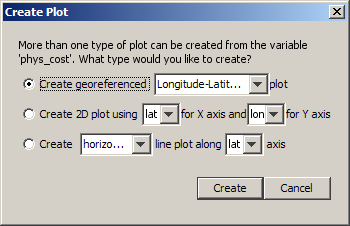
\includegraphics[scale=2.0]{CreatePlot.png}
\end{center}
\caption{\textbf{Panoply} \textsf{Create Plot} dialogue window.}
\label{fig:CreatePlot}
\end{figure}

You can interpolate the data or not (often you may find that it is clearer not to interpolate the data but to leave it as 'blocky' colors corresponding to the resolution of the model), change the scale and colors, overlay continental outline, change the projection, etc etc. Gray cells represent 'dry' grid points, i.e., continental or oceanic crust.
To save plots in \textbf{Panoply} -- from the file menu: \footnotesize\textsf{File}\normalsize, then \footnotesize\textsf{Save Image As ... }\normalsize and then select the location, filename, and graphics format.

%------------------------------------------------

\subsection{Issues with Panoply default settings}

The default settings in \textbf{Panoply}, i.e. those used when a plot is first created, can often mislead. In particular, note:
\begin{itemize}

\vspace{1mm}
\item \footnotesize\textsf{Year }\normalsize (\footnotesize\textsf{Array}\normalsize tab)
        \\ The default is for the very 1st \textit{time-slice} to be displayed rather than the experiment end. The first \textit{time-slice} is numbered from 1 to however many total time-slices have been saved (displayed to the immediate right of the \footnotesize\textsf{Year ,}\normalsize box), and it is this integer number that appears in the \footnotesize\textsf{Year }\normalsize box -- not the year of the data save. Instead, the mid-point year of the time-slice is displayed in a second box (labeled '\footnotesize\textsf{Year mid-point}\normalsize').
        \\ Different \textit{time-slices} to be plotted can be selected by either clicking through the saved year count, or by selecting the save year mid-point from the drop-down list.

\vspace{1mm}
\item \footnotesize\textsf{Scale Range }\normalsize (\footnotesize\textsf{Scale}\normalsize tab)
        \\ The color scale is auto-scaled so that the range always goes from the minimum to maximum displayed value. This can potentially mislead if save years and/or depth/latitude slices are scrolled through as the scale will be automatically adjusted to fit each plot in turn.
        \\ Confusion can also arise for fields with no variation, e.g. atmospheric trace gas concentrations or air temperature -- the auto-scaled plot in these instances has a uniform color but with odd hatching as Panoply dutifully tries to achieve the impossible (creating a scale of multiple colors for a single value).

\vspace{1mm}
\item Zonal averaging (\footnotesize\textsf{Array }\normalsize tab)
        \\ \footnotesize\textsf{Lat-Vert }\normalsize plots are displayed as a zonal mean by default. This is indicated by the tick in the \footnotesize\textsf{Ave }\normalsize box (bottom RH corner). Un-ticking the \footnotesize\textsf{Ave }\normalsize box releases the averaging with the first longitudinal value of the grid now displayed instead. Similar to how Panoply displays years -- the longitudinal grid locations are counter from 1 to typically 36 (depending on the resolution of the ocean grid), with the longitudinal mid-point value in degrees East displayed to the right.
        \\ Different longitudinal sections to be plotted can be selected by either clicking through the grid point number count, or by selecting the longitudinal mid-point from the drop-down list.

\vspace{1mm}
\item Scale bar tick marks (\footnotesize\textsf{Array }\normalsize tab)
        \\ The tick labels on the color scale are displayed by default in the format: \footnotesize\textsf{x.y }\normalsize. If the typical values of the variable are order e.g. 10\begin{math}^{-6}\end{math} you will end up with value labels ranging from \footnotesize\textsf{0.0 }\normalsize to \footnotesize\textsf{0.0 }\normalsize ... This can be most easily resolved in one of two ways:
        \begin{itemize}
\item The format of the label can be changed by selecting a different option from the pull-down \footnotesize\textsf{Tick Label Format }\normalsize box (default == \footnotesize\textsf{\%.1f}\normalsize). For instance, \footnotesize\textsf{\%.2e }\normalsize would give a display in the format \footnotesize\textsf{x.xxEyy }\normalsize (or \footnotesize\textsf{x.xxE-yy}\normalsize) or \footnotesize\textsf{\%.6f }\normalsize would give \footnotesize\textsf{x.xxxxxx}\normalsize.
\item An alternative is to re-scale the values. This is done in the Scaling Factor box in which you set the scale factor in powers of 10. For example: setting \footnotesize\textsf{-6}\normalsize in effect converts units of mol kg\begin{math}^{-6}\end{math} to \begin{math}\mu\end{math}mol kg\begin{math}^{-6}\end{math}.
\end{itemize}

\vspace{1mm}
\item Other things to watch out for include:
\begin{itemize}
\item A plot involving depth, being by default, 'up-side-down'!.
\\This is fixed in the \footnotesize\textsf{Grid}\normalsize tab, and the click button, \footnotesize\textsf{Swap B/T}\normalsize.
\item In \footnotesize\textsf{'Lon-Lat'}\normalsize plots, the modern continental outline being displayed by default.
\\This can be fixed by changing options in the \footnotesize\textsf{Overlay}\normalsize tab.
\end{itemize}

\end{itemize}
\vspace{2mm}

\begin{center}
\textbf{Simply be careful when opening a new plot that you are looking at what you *think* you are looking at (or what you think you are looking at *is* what you are looking at).}
\end{center}

Note that default plotting settings in \textbf{Panoply} can be changed (and saved).

%------------------------------------------------

\subsection{Basic plots -- examples}

\vspace{1mm}
\noindent\rule{4cm}{0.5pt}
\vspace{2mm}

\noindent\textcolor{red}{TO COME ...}

\vspace{1mm}
\noindent\rule{4cm}{0.5pt}
\vspace{2mm}

%------------------------------------------------

\subsection{Difference (anomaly) plots}

It is possible to create an anomaly (difference) maps in \textbf{Panoply} which are essential when analyzing changes in a variable that may be small compared to the global spatial variability. To do this:

\begin{itemize}
\vspace{1mm}
\item First, open the netCDF results file.
\vspace{1mm}
\item Open the variable of interest, e.g., \texttt{atm\_temp} (surface air temperature) in the 2D netCDF file.
\vspace{-4mm}
\item From the upper LH corner of the Dataset Browser window, from the drop-down menu, select the name of the plot you have just created (\texttt{atm\_temp} in \footnotesize\textsf{field\_biogem\_2D}\normalsize ...).
\vspace{1mm}
\item From the upper LH corner of the Dataset Browser window, now click on the \footnotesize\textsf{Combine Plot}\normalsize icon.
\\ You now have a plot window that is displaying a difference map. By default, it is showing you the difference between two identical (in time) slices. The two different slices are labeled Array 1 (LH side) and Array 2 (RH side).
\\NOTE: Easier than mucking about with \footnotesize\textsf{Combine Plot}\normalsize, is having open the first dataset, simply drag another variable from the list of variables in the \footnotesize\textsf{Sources }\normalsize window, into the \footnotesize\textsf{Plot }\normalsize window. You can drag either a different, or the same variable, into the \footnotesize\textsf{Plot }\normalsize window.
\end{itemize}
\vspace{2mm}

For instance, you can keep one array (Array 1) fixed to the initial (year 1 (centered on 0.5)) and vary the year in the second array (Array 2). Note that you can select in Panoply whether Array 1 - Array 2 is plotted, or Array 2 - Array 1, or various proportional or relative differences.

If you switch off the auto-scaling feature (\footnotesize\textsf{Always fit to data}\normalsize) you can center the scale so that no change is white, with positive deviations = red and negative = blue by clicking on Center on 0. This is something of a convention in the scientific literature.

The same variable in two different model experiments can also be opened up and analyzed combined:

\begin{itemize}
\vspace{1mm}
\item Start by opening up both required netCDF files.
\vspace{1mm}
\item Open the variable of interest in one (either one) of the two 2D netCDF data-sets.
\vspace{1mm}
\item From the upper LH corner of the Dataset Browser window, from the drop-down menu, select the name of the plot you have just created.
\vspace{1mm}
\item Now double-click in the variable in the 2nd netCDF dataset.
\\ You now have a plot window that is displaying a difference map, but of the same variable between two different experiments, rather than two years of the same experiment.
\end{itemize}
\vspace{2mm}

%------------------------------------------------

\subsection{Ocean velocity plots}

By combining the two (horizontal) fields of ocean circulation, rather than a difference plot, \textbf{Panoply} can create a velocity plot. This is a great way of visualizing surface (and deeper) currents and circulation patterns. To do this:

\begin{itemize}
\vspace{1mm}
\item First, open the 3-D netCDF results file.
\vspace{1mm}
\item Open either the \texttt{phys\_u} ('ocean velocity - u') or \texttt{phys\_v} ('ocean velocity - v') field and select a \footnotesize\textsf{Lon-Lat }\normalsize plot.
\vspace{1mm}
\item From the upper LH corner of the \footnotesize\textsf{Sources }\normalsize window, from the drop-down menu, select the name of the plot you have just created.
\vspace{1mm}
\item Now double-click on the other velocity variable (whichever of the u and v fields you did not open first).
\vspace{1mm}
\item By default you get a difference map, which is pretty useless really. From the drop-down \footnotesize\textsf{Plot }\normalsize menu box (which should be displaying 'Array 1 - Array 2' by default) select: \footnotesize\textsf{Vector Magnitude }\normalsize(bottom of the list).
\\ You now have a plot window that is displaying the ocean velocity field, with arrows indicating the direction and speed (length of the arrow) together with an interpolated color background of the speed.
\end{itemize}
\vspace{2mm}

You can re-scale the velocity arrows to more clearly display the circulation pattern by altering the \footnotesize\textsf{Scale Length }\normalsize value (\footnotesize\textsf{Contours \& Vectors }\normalsize tab). A value of 0.1 is a reasonable choice for surface currents. e.g. see Figure \ref{fig:cgenie_currents}.

If you want to display deeper (in the ocean) current fields and/or different time-slices, take care that the depth level (/time-slice) in both LH and RH sides of the \footnotesize\textsf{Array(s) }\normalsize panel must be changed to the same value. If displaying deeper current fields, then the velocity vectors will have to be further re-scaled (to a smaller value) in line with the lower velocities at depth compared to the surface.

\newpage

\begin{figure}[ht]
\begin{center}
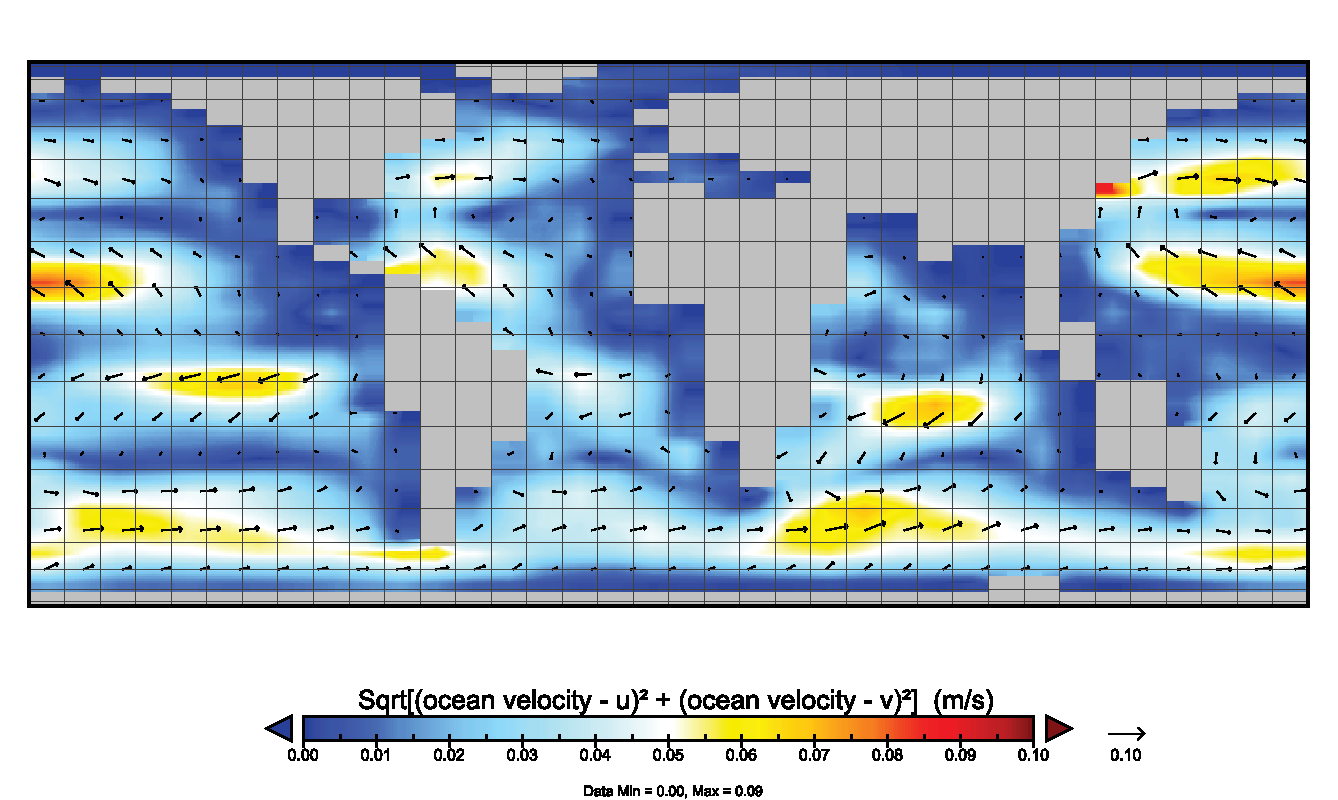
\includegraphics[scale=0.5]{cgenie_currents.pdf}
\end{center}
\caption{Example (modern) ocean surface velocity (current) map.}
\label{fig:cgenie_currents}
\end{figure}

%------------------------------------------------

\newpage

%------------------------------------------------

\section{MATLAB plotting}

%------------------------------------------------

\subsection{MATLAB 101}

If you need a tutorial on \textbf{MATLAB}, either as a refresher, or because you have not used the program before, refer to (and/or work through) the following sections of the \href{https://github.com/derpycode/matlabananas\#matlabananas}{matlabananas} \textbf{MATLAB} textbook:

\vspace{2pt}
\begin{itemize}
\vspace{1pt}
\item Chapter 1 --  this covers the very basics of using \textbf{MATLAB}, what variables are, including scalars (e.g. single numbers), vectors (1D array), matrices (2D array) and higher order arrays, now to index and carry out basic manipulation of arrays, basic data loading and saving and plotting.
\vspace{1pt}
\item Sections 2.1 and 2.2 of Chapter 2, which cover creating (script) programs -- i.e. adding all your \textbf{MATLAB} commands to a file (a \footnotesize\textsf{.m }\normalsize or '\footnotesize\textsf{m-file }\normalsize') and running the file, and \textit{functions} -- programs (\footnotesize\textsf{m-file}\normalsize s) where one or more parameters might be passed into the \textit{function} when it is called (e.g. at the command line), and potentially variables returned.
\vspace{1pt}
\item In Chapter 3 -- subsection 3.1.3 deals with reading in netCDF format data, which is the \textbf{muffin} format for spatial data. Section 3.2 deals with more advanced 2D plotting (also of direct relevance to \textbf{muffin} data processing and visualization using \textbf{MATLAB}).
\end{itemize}
\vspace{2pt}

%------------------------------------------------

\subsection{MATLAB and ASCII (\textit{time-series})}

The \textit{time-series} (\textsf{\footnotesize .res}) output of \textbf{BIOGEM} are in a simple plain text (ASCII) format. These can be read in very easily in \textbf{MATLAB} using the \texttt{load} command. Note that a brief description of each column of data in the \textit{time-series} files appears on the first first line of the file, and that prefixing this is a \texttt{\%} symbol, that \textbf{MATLAB} ignores. Hence only the columns of data gets read in by default using \texttt{load} :) \footnote{There are also other \textbf{MATLAB} commands for reading in text data -- refer to to the \href{http://www.seao2.info//teaching/201718.GEO111/GEO111.pdf}{\textbf{MATLAB} programming text}.} For example:

\small\begin{verbatim}
>> co2=load('biogem_series_atm_pCO_2.res','-ascii');
>> plot(co2(:,1),1.0E6*co2(:,3));
\end{verbatim}\normalsize

\noindent loads in the atmospheric \(CO_{2}\) time-series file (assigning it to the array variable \texttt{co2}), and then plots (as a line graph) the 3rd column (\(CO_{2}\) concentration) vs. the first (time). Because concentrations are saved in units of atmospheres, a factor of \texttt{1.0E6} is applied to concert to \(\mu atm\). Equivalently:

\small\begin{verbatim}
>> co2=load('biogem_series_atm_pCO2\).res','-ascii');
>> scatter(co2(:,1),1.0E6*co2(:,3));
\end{verbatim}\normalsize

%------------------------------------------------

\subsection{MATLAB 'Import Data' ...}

You can also import the time-series files by clicking on the \footnotesize\textsf{Import Data }\normalsize icon:

\begin{itemize}
\vspace{1pt}
\item Navigate to the \textbf{BIOGEM} sub-directory of your experiment results directory. Ensure that \footnotesize\textsf{All Files }\normalsize is selected and click on the time-series file you want.
\vspace{1pt}
\item \textbf{MATLAB} ignores the header lines, and it should be safe to simply click on \footnotesize\textsf{Import Selecftion }\normalsize for all columns, or select what you want to plot -- typically year (the first column) and another one.
\vspace{1pt}
\item A default variable name -- the filename minus the underscore characters -- will appear listed in the \textbf{MATLAB} \footnotesize\textsf{Workspace window }\normalsize. Double-click on the variable name to open up the imported data in a table view. If you select columns to plot, and then head over to the main \footnotesize\textsf{PLOTS }\normalsize tab, a range of plotting options are provided and a plot can be generated by clicking on one of the plotting icons.\footnote{Note that if you have not selected any data columns, then all the plotting icons are disabled and greyed out in the \footnotesize\textsf{PLOTS }\normalsize tab.}
\vspace{1pt}
\item Labels can be added, scales and markers changed, etc etc, in the \footnotesize\textsf{Figure window }\normalsize.
\end{itemize}
\vspace{2pt}

Note that as the data has been imported as an array in \textbf{MATLAB}, you can also plot directly from the command line. (And indeed, you could also have loaded the data from the command line.)

%------------------------------------------------

\subsection{MATLAB and netCDF (\textit{time-slice})}

\noindent Basically -- the only hard part, having opened the \textit{netCDF} file is in correctly deducing which dimension in an extracted data array is   longitude, latitude, (sometimes depth), or time. Mostly this should be pretty obvious from inspecting the \textbf{MATLAB} \footnotesize\textsf{Workspace }\normalsize window (assuming you have a column for \footnotesize\textsf{Size }\normalsize selected to be displayed), or using the \texttt{size} command.\footnote{It also turns out that the order of dimensions for a variable read in by \textbf{MATLAB}, is the opposite of the order listed in the \textsf{Variable} window of \textbf{Panoply}.} Once you have done this, you can plot slices, scale data, average or otherwise process data, extract locations at specific locations, etc etc.

As an example -- in \textbf{MATLAB}, first either change directory to the \textsf{\small biogem} directory of a set of \textbf{muffin} results, or from where-ever you are, add a path to the location of the \textsf{\small biogem} directory. To open the 2D \textbf{BIOGEM} netCDF results file, type:
\begin{verbatim}
>> ncid = netcdf.open('fields_biogem_2d.nc','nowrite');
\end{verbatim}

To extract a variable, you first need to find its ID from its name:
\begin{verbatim}
>> varid = netcdf.inqVarID(ncid,NAME);
\end{verbatim}
where \texttt{NAME} is a place-holder for the name of he variable (as a string). You might need to use \textbf{Panoply} to display all the different variable names. Or, you can list all the variables and stuff in the netCDF file using \texttt{ncdisp}:
\begin{verbatim}
>> ncdisp('fields_biogem_2d.nc')
\end{verbatim}

Having, by one means or another, identified the name of the variable you are interested in, you can recover its ID and then the data itself, for example, for \textsf{\footnotesize atm\_temp} (\textsf{\footnotesize surface air temperature}):
\begin{verbatim}
>> varid = netcdf.inqVarID(ncid,'atm_temp');
>> data  = netcdf.getVar(ncid,varid);
\end{verbatim}

In loading in the variable, you end up with a multi-dimensional array -- 2 spatial dimensions and if you have more than 1 \textit{time-slice} of data saved, 1 temporal dimension (and if you loaded in the \textbf{BIOGEM} 3D netCDF file, you end up with a 4-dimensional array). \textbf{MATLAB} reports the size of the array in the \textsf{\footnotesize Workspace window} (depending on which column display options you have selected). In the example here, which took the experiment \textsf{\footnotesize EXAMPLE.worjh2.Caoetal2009.RCP6p0}, the array for atmospheric temperature is reported as \(36\times36\times8\).\footnote{Although note that in \textbf{Panoply}, it is reported as \textsf{\scriptsize atm\_temp(time=8, lat=36, lon=36)}.} so the last of the 8 time-slices would  be accessed as:
\begin{verbatim}
>> data_last = data(:,:,8);
\end{verbatim}
or
\begin{verbatim}
>> data_last = data(:,:,end);
\end{verbatim}

Panoply reports variables in the the \textbf{BIOGEM} 3D netCDF file as having dimensions of: (\textit{time, zt, lat, lon}) (e.g. (time=13, zt=16, lat=36, lon=36)) whereas \textbf{MATLAB} reads it in the reverse order. For instance, if we load in the (3D) ocean temperature field:
\begin{verbatim}
>> ncid = netcdf.open('fields_biogem_3d.nc','nowrite')
>> varid = netcdf.inqVarID(ncid,'ocn_temp');
>> data  = netcdf.getVar(ncid,varid);
\end{verbatim}
and then type:
\begin{verbatim}
>> size(data)
ans =
    36    36    16    13
\end{verbatim}
we get an array orientated as (\textit{lon, lat, zt, time}).\footnote{\textit{zt} is the depth level in the ocean.} The final time-slice would hence then be accessed:
\begin{verbatim}
>> data_last = data(:,:,:,end);
\end{verbatim}
with \texttt{data\_last} now becoming a 3D array with dimensions (\textit{lon, lat, zt}).

\vspace{2mm}
There are three key things to remember at this point:

\begin{enumerate}
\setlength{\itemindent}{.2in}

\vspace{1mm}
\item Firstly, the depth levels are read such that index \texttt{1} is the surface, and \texttt{16} is the deepest ocean depth level (in this case, otherwise it is \texttt{8}).

\vspace{1mm}
\item For the lon-lat part -- (\textit{lon, lat}) equates to \textit{row}\textit{}s vs. \textit{columns} in \textbf{MATLAB}, and hence if you were to plot e.g. the surface ocean slice:
\begin{verbatim}
>> imagesc(data_last(:,:,1));
\end{verbatim}
you will end up with the plot on its side, with latitude along the \textit{x}-axis and longitude on the \textit{y}-axis.
\\You can exchange rows and columns in \textbf{MATLAB} with the \textit{transpose operator} (see programming/\textbf{MATLAB} book):
\begin{verbatim}
>> imagesc(data_last(:,:,1)');
\end{verbatim}
but ... this still leaves you with an up-side-down plot, because \textbf{MATLAB} reads from the first row down, whereas in latitude, you are expecting to read from -90 degrees up (towards the N pole). \texttt{flipud} accomplishes the final transformation:
\begin{verbatim}
>> imagesc(flipud(data_last(:,:,1)'));
\end{verbatim}

\vspace{1mm}
\item The final complication is that \textbf{muffin} netCDF output uses a special value to represent an invalid or null number, e.g. for ocean temperature where the grid point is land (and an ocean temperature value would have no meaning). In the netCDF definition, \textbf{Panoply} is told what the special number is, hence it shows land in grey when plotting ocean variables.

Panoply reports this as: \textsf{\footnotesize missing\_value = 9.969209968386869E36}.

\vspace{1mm}
There is no easy way (that I can see!) to get \textbf{MATLAB} to deal with this for you, so you need to search and replace this value, e.g.:
\small\begin{verbatim}
>> null=9.969209968386869E36;
>> data_last(find(data_last==null))=NaN;
\end{verbatim}\normalsize
which searches for this null value and replaces it with a \texttt{NaN} (so that now it can be simply plotted).

\end{enumerate}
\vspace{2mm}

Once you are done accessing data, it is good practice to close the netCDF file after you are done with it:
\begin{verbatim}
>> netcdf.close(ncid);
\end{verbatim}

The question then remains: what do you actually 'do' with it in \textbf{MATLAB}?

%------------------------------------------------

\subsubsection{Plotting sections}

For a quick look-see, \texttt{imagesc} (as per above) is handy.

\noindent For more advanced plotting (and for presentation) -- refer to the \textbf{matlabananas} \textbf{MATLAB} programming text.

\noindent As per above, horizontal (lon-lat) fields can be extracted from 2D \textit{netCDF} output by: \texttt{data(:,:,time)} and from 3D by: \texttt{data(:,:,zt,time)}. Obviously, you could also extract lon-depth via: \texttt{data(:,lat,:,time)} and lat-depth via: \texttt{data(lon,:,:,time)}.

\noindent Anomalies (with time) are created: \texttt{data(:,:,:,time2)-data(:,:,:,time2)}.

Typically, except a little trial-and-error in extracting the dimensions you want, and also in correcting the orientation of the matrix or resulting plot.

%------------------------------------------------

\subsubsection{Calculating inventories}

Often, the inventory (total mass or number of moles) of the ocean or atmosphere is useful to know, particularly as a function of time. For the ocean (or atmosphere) as a whole, the \textit{time-series} output files report this (alongside the mean global concentration).

You can also calculate this with \textbf{MATLAB} from the netCDF output. Fields of ocean concentration are saved in the 3D output (and atmospheric concentrations in the 2D output). To convert concentration in the ocean, in units of \(molkg^{-1}\) you'll need to know the mass of each ocean cell, in units of \(kg\).

When saving using save option \texttt{9}, or \texttt{99}\footnote{Parameter \texttt{bg\_par\_data\_save\_level} -- see earlier.}, you save the 'physics' of the ocean model, which is actually mostly just the grid information, such as cell area, thickness, latitude and longitude edges and midpoints, depth edges and mid point. Also saved are the masses and volumes of the grid of cells. So to derive an array of cell tracer inventories from an array of concentrations, and the array of cell masses (variable \textsf{\footnotesize phys\_ocn\_M}), you'd write:

\pagebreak

\small\begin{verbatim}
varid = netcdf.inqVarID(ncid,'ocn_temp');
data  = netcdf.getVar(ncid,varid);
varid = netcdf.inqVarID(ncid,'phys_ocn_M');
mass  = netcdf.getVar(ncid,varid);
inventory = data(:,:,:,time).*mass(:,:,:,time);
\end{verbatim}\normalsize
\noindent Before summing \texttt{inventory} to determine the global total inventory, you will, as before, have to deal with the null values (converting them to \texttt{NaN}) and then deal with the presence of \texttt{NaN}s in the array when summing ...

The advantage of doing the calculations in \textbf{MATLAB} (despite being provided with the global mean and inventory in the time-series files) is that you could calculate the inventory of a tracer (/substance) for just the ocean surface, or just a specific region of band of latitude. Or you could calculate the mean concentration for just a specific region of the ocean.\footnote{In calculating mean concentrations, you'll need to volume or mass weight the concentrations, and hence still need to use one of the physics variables.}

%----------------------------------------------------------------------------------------
%----------------------------------------------------------------------------------------